\documentclass[10pt,a4paper]{book}
\usepackage{hyperref}
\usepackage{parskip}
\usepackage{listings}
\usepackage{color}
\usepackage{amsmath}
\usepackage{alltt}
\usepackage[pdftex]{graphicx}
\usepackage{graphviz}
\usepackage{multirow}
\usepackage{graphicx}
\usepackage{epstopdf}
\usepackage{geometry}
\geometry{bindingoffset=1cm}

\usepackage{float}
\floatstyle{boxed} 
\restylefloat{figure}

\usepackage[toc]{glossaries}

\begin{document}
\newcommand{\sups}[1]{\ensuremath{^{\textrm{#1}}}}
\newcommand{\subs}[1]{\ensuremath{_{\textrm{#1}}}}
%\newcommand{\lam}[0]{\ensuremath{\textrm{\lambda}}}

\lstset{
  language=caml,
  basicstyle=\scriptsize,
  upquote=true,
  aboveskip={1.5\baselineskip},
  columns=fixed,
  showstringspaces=false,
  extendedchars=true,
  breaklines=true,
  prebreak = \raisebox{0ex}[0ex][0ex]{\ensuremath{\hookleftarrow}},
  frame=single,
  showtabs=false,
  showspaces=false,
  showstringspaces=false,
  identifierstyle=\ttfamily,
  keywordstyle=\color[rgb]{0,0,1},
  commentstyle=\color[rgb]{0.133,0.545,0.133},
  stringstyle=\color[rgb]{0.627,0.126,0.941},
}
\setcounter{tocdepth}{1}
\newglossaryentry{js}
{
  name=JavaScript
  description={is a scripting language used for web applications.}
}

\makeglossaries


  \frontmatter
  \begin{titlepage}
  \begin{flushright}
    Henry Hughes
  \end{flushright}
  \vspace{2.0in}
  \begin{center}
    \Huge Functionally Reactive Web Applications
  \end{center}
  \vfill
  \begin{center}
    \large Computer Science Tripos
  \end{center}
  \vspace{0.1in}
  \begin{center}
    \large Jesus College
  \end{center}
  \vspace{0.1in}
  \begin{center}
    \large 2011
  \end{center}
\end{titlepage}

  \chapter{Proforma}

  \chapter{Declaration of Originality}
I \emph{Henry Hughes} of \emph{Jesus College}, being a candidate for Part II of the Computer Science Tripos, hereby declare that this dissertation and the work described in it are my own work, unaided except as may be specified below, and that the dissertation does not contain material that has already been used to any substantial extent for a comparable purpose.

Signed 

\vspace{0.4in}

Date

  \tableofcontents

  \mainmatter
  \chapter{Introduction}

This chapter introduces the reasons for the project and the goals it sets out to achieve. It looks at the advantages of web applications and some of the issues currently involved in developing them.

\section{Motivation}
Web applications are becoming increasingly popular due to the disadvantages associated with applications installed on the local machine. One such issue is that the software is difficult to upgrade. Another is that it often costs the user a large one-off amount because it is difficult for the vendor to maintain a service contract when they have distributed a copy of the software binary to the user. If these applications are instead hosted from a remote server then the vendor can worry about upgrading and updating the software and can charge a much smaller but regular fee to the user for the service~\cite{bib:road_ahead}.

There is a variety of programming languages which can be used to create desktop applications. Each provides certain advantages so the developer can choose the language which best suits their needs; this could be anything from the run-time guarantees the programming language provides to rapid development and prototyping. It does not make much difference to the user which language is used; all they want to do is run their favourite application. When writing an application for the Web, however, the programmer is forced to use a specific set of tools. These tools come under the umbrella term \emph{AJAX} (Asynchronous JavaScript and XML). AJAX involves writing client-side code in JavaScript and performing asynchronous requests to the server. This provides a more interactive environment than the classical web application model. The classical model uses the server to create the next web page on the fly and then reloads the current page with the new one. This is often less desirable than AJAX because loading the new page causes a break in the user's work flow~\cite{bib:ajax}.

While JavaScript is a full-featured language, there are other programming languages which provide features it does not. It would be nice if those other languages could be used to write web applications without having to provide a new environment to run them in. In that way, the applications could be written in the developers language of choice but then compiled into JavaScript so would run in current web browsers.

The purpose of this project is to explore the usefulness of writing web applications using \emph{functional} and \emph{reactive} programming techniques.

\section{Concepts}

This section gives a brief overview and some examples of some programming concepts which lead to functional reactive programming (FRP).

\subsection{Glossary of Terms}

\textbf{Imperative Programming}: \emph{A programming language which uses a series of statements to manipulate an implicit state}~\cite{bib:prog}.

\textbf{Declarative Programming}: \emph{These languages are designed to have no state and no assignment. Any state has to be passed into functions as parameters}~\cite{bib:prog}.

\subsection{Scripting Languages}
Scripting is a special type of imperative programming. Scripts are commonly used in rapid prototyping and for performing simple tasks and computations. They often use lazy typing and have minimal structure. JavaScript is a scripting language with C-like syntax which has been adopted by web developers as the most prominent way to perform client-side programming in web applications~\cite{bib:crockford}.

\subsection{Functional Programming}
\label{lab:functional}
The functional programming languages are a subset of the declarative programming languages. With functional programming, \emph{functions} are used as the underlying computation model. Some of the key features of functional programming languages include strong static typing, type inference and polymorphism. These guarantee that any program which passes the type inferencer will not have any type errors~\cite{bib:functional_prog}.

\subsection{Reactive Programming}
Reactive programming provides a way to express how data flows through a program. With imperative programming, if the result of a calculation is assigned to a variable, a change to the inputs of that calculation will not alter the value stored. With reactive programming, however, changes to inputs are passed through the program. Thus the values of variables can depend on the values of other variables and inputs and will update accordingly. Reactive programming languages construct a data-flow graph whose nodes are the variables in the program and whose edges are the dependencies for each variable~\cite{bib:functional_react,bib:lowering}. There are several examples of reactive programming languages. One such example is \emph{ESTEREL}, which is used for programming reactive systems in hardware~\cite{bib:esterel}. Another is \emph{flapjax} which is a language for writing reactive web applications in JavaScript~\cite{bib:flapjax}.

Functional reactive programming is a combination of these two concepts, writing reactive programs using a functional programming language. An example of functional reactive programming can be seen \emph{Functional Reactive Animation}~\cite{bib:fran}.

\section{Purpose}
\label{lab:goals}
The goals of this project are to find solutions to the following questions:

\emph{Is compiling JavaScript pages from a functional programming language a good idea? Where is it useful and what are the downsides?}

\emph{Is reactive programming useful in the context of web applications? Is there a particular situation where the gains (in terms of both computation and code production efficiency) are particularly great?}

  \chapter{Preparation}

\section{Starting Point}

\subsection{JavaScript}
JavaScript is used for client-side scripting on web pages. It is run on the local machine inside the browser environment and can access and modify the Document Object Model (\emph{DOM}), the browsers representation of the  objects on the current web page. By manipulating the DOM at run-time, JavaScript can be used to make interactive user interfaces and dynamic pages.

\subsection{OCaml}
Caml (Categorical Abstract Machine Language) is a general purpose language which supports functional, imperative and object-oriented programming styles. It features a powerful type system which uses parametric polymorphism and type inference. This allows methods to be designed without having to explicitly declare the types of parameters or the result so functions can be reused on many different types of inputs. It also has pattern matching which can be used to direct control flow of the program through functions depending on their inputs.\cite{bib:caml}

OCaml (Objective Caml) is a variant of the Caml language. It is an extension of Caml which adds an object-oriented layer and module system. It is designed for use in developing commercial systems and is the most popular Caml derivative.\cite{bib:ocaml}

\subsection{JavaScript vs OCaml}
In some ways JavaScript is very similar to OCaml. In both languages functions are first class objects, they can be assigned to variables, passed as function parameters and invoked. However the typing systems of OCaml and JavaScript are very different. OCaml types start off generic and get more specific each time they are used. In JavaScript variables themselves do not have a type and so can be reassigned to a value of any type. This can lead to programming errors because you are not guaranteed to know the type of your object at any point. Another difference is that OCaml is checked for errors at compile-time where as JavaScript is checked at run-time. If a piece of code is not executed in a test-run you cannot be sure that it will succeed.

\section{Requirements Analysis}
A successful implementation of this project should:
\begin{itemize}
\item Provide two or more significantly different web applications.
\item These applications must be cross-browser compatible.
\item Each must make use of ocamljs and froc.
\item ...
\end{itemize}

\section{Tools}

\subsection{ocamljs}
ocamljs is a modified version of the OCaml compiler. It uses the standard OCaml compiler up to the point when lambda code is generated, it replaces the last stage where bytecode is generated and outputs JavaScript instead. Figure \ref{fig:ocamlc} shows the stages of the OCaml compiler and ocamljs. \cite{bib:oreilly}

\begin{figure}
  \center{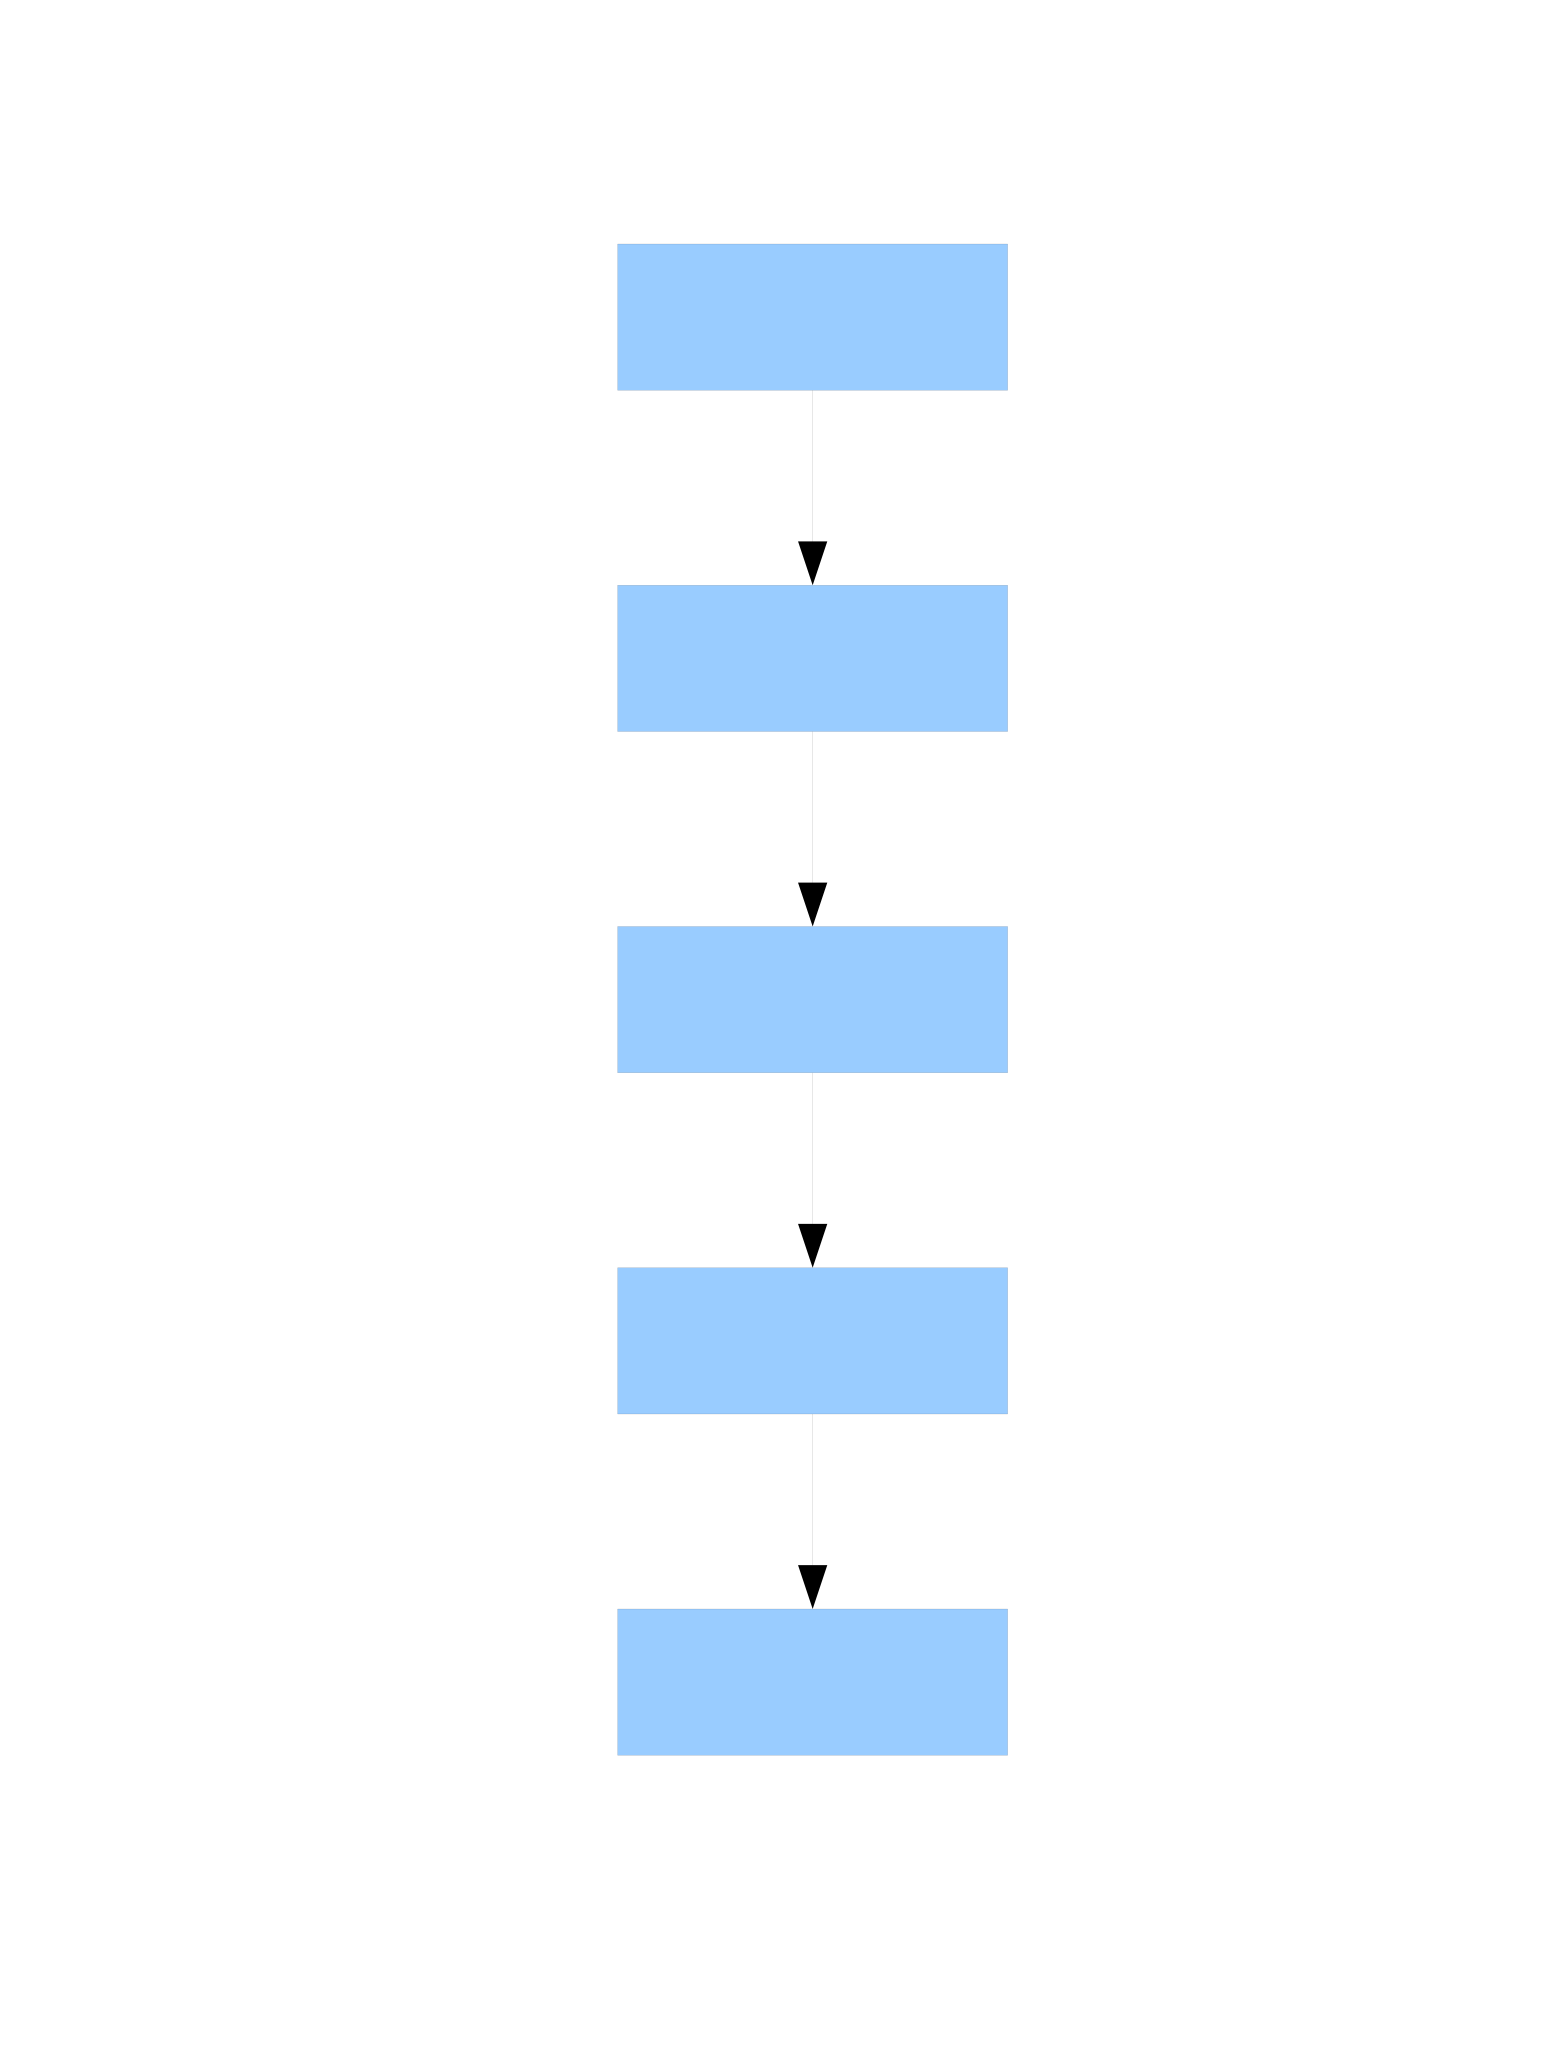
\includegraphics[scale=0.5]{images/ocamlc.pdf}}
  \caption{Stages of the OCaml compiler (ocamlc) and ocamljs.\cite{bib:oreilly}}
  \label{fig:ocamlc}
\end{figure}

\subsubsection{Lambda Code}
Lambda code is based on the $\lambda-calculus$. This notation was invented by Alonso Church in the 1930s. It is used to describe the most basic ways operators and functions can be combined. Conversion from mathematical functions to lambda-expressions is fairly straight forward. Here is a short example:\cite{bib:lambda}

$f(x) = x - 1$ becomes $\lambda.x x-1$

This may not look like a big change but it provides a systematic notation which is good for incorporation into programming. When there are multiple parameters for a function, instead of having a multi-parameter lambda-expression multiple single parameter lambda-expressions are chained. For example:

$\lambda.y \lambda.x x - y$.

Lambda code is very similar to $\lambda-calculus$. Consider the following OCaml program:

\begin{alltt}
let f a b = a+b
let three = f 1 2;;
\end{alltt}

The OCaml compiler can output the lambda representation if the \emph{-dlambda} command-line switch is used. This is the lambda output for the above OCaml:

\begin{alltt}
  (setglobal Simple!
  (let (
  f/58 (function a/59 b/60 (+ a/59 b/60))
  three/61 (apply f/58 1 2))
  (makeblock 0 f/58 three/61)))
\end{alltt}

In this lambda code variables have been renamed. The lambda-expression part is \emph{function a/59 b/60 (+ a/59 b/60)} which is equivalent to \texttt{$\lambda a.\lambda b.a+b$}.

\subsubsection{Lambda to JavaScript}
Functions and exceptions map simply into JavaScript. Integers and floats can be represented as a JavaScript \emph{number} and booleans by the JavaScript \emph{bool}. The standard library functions have been reimplemented in a static JavaScript file.\cite{bib:js_comp}

\subsubsection{Function Applications}
Function applications are a bit more tricky. Functions in JavaScript require the correct number of arguments but in OCaml, functions can receive more (\emph{tail calls}) or less arguments (\emph{partial application}). When we have a partial application we want to return a closure and when we have a tail call we want to apply the extra arguments to the result. This is solved using Simon Peyton Jones' \emph{eval-apply} method.\cite{bib:js_comp,bib:krivines_machine}

\subsubsection{Eval-Apply}
With this scheme the caller is responsible for providing the correct number of arguments to a function. If there are not enough a closure has to be created and if there are too many the left over arguments are applied to the result of the function. This is implemented using the \emph{apply} function outlined in Figure \ref{eval-apply}.\cite{bib:krivines_machine}

\begin{figure}
  \begin{alltt}
f a\subs{1} ... a\subs{n} -> apply\subs{n}(f, a\subs{1}, ..., a\subs{n})

apply\subs{n} = \lam f x\subs{1} ... x\subs{n}
  match arity(f) with
    | 1   -> apply\subs{n-1} (f(x\subs{1}), x\subs{2}, ..., x\subs{n})
    | ...
    | n-1 -> apply\subs{1} (f(x\subs{1}, ..., x\subs{n}), x\subs{n})
    | n   -> f(x\subs{1}, ..., x\subs{n})
    | n+1 -> papp\subs{n+1,n}(f, x\subs{1}, ..., x\subs{n})
    | n+2 -> papp\subs{n+2,n}(f, x\subs{1}, ..., x\subs{n})
    | ...

papp\subs{p,q} = \lam f x\subs{1} ... x\subs{q}. (\lam x\subs{q+1} ... x\subs{p}. f(x\subs{1}, ..., x\subs{p}))
  \end{alltt}
  \caption{Eval-apply implementation}
  \label{eval-apply}
\end{figure}

\subsubsection{ocamljs Example}
Consider a simple function which takes two arguments and returns the summation of them and then an application of this function. Figure \ref{example} shows the OCaml code and compiled JavaScript for this example.

\begin{figure}
  \begin{tabular}{| p{4cm} | p{7.3cm} |}
    \hline
    \textbf{OCaml} & \textbf{JavaScript}\\ \hline
    \begin{alltt}
let f a b = a+b
let three = f 1 2;;
    \end{alltt}
    &
    \begin{alltt}
function () \{
  var f\$58 =
    _f(2, function (a\$59, b\$60) \{
      return a\$59 + b\$60;
    \});
  var three\$61 = _(f\$58, [ 1, 2 ]);
  return \$(f\$58, three\$61);
\}
    \end{alltt} \\ \hline
  \end{tabular}
  \caption{OCaml source and JavaScript output example}
  \label{example}
\end{figure}

\subsection{froc}

\emph{froc} is an OCaml library for reactive programming in OCaml.

\subsubsection{Self Adjusting Computation}
froc uses \emph{self adjusting computation} to push updates to input variables through data paths in the program. Self adjusting means that once the variable has been defined, the program will automatically forward changes to dependencies. This is stored by the program as a \emph{dependency graph}.

\subsubsection{Dependency Graphs}
Given a set of variables and another set of variable dependencies (pairs of variable) a directed graph can be created where the variables form the nodes and the dependencies are the edges. This is a dependency graph and it is used by reactive programs to describe data-flow throughout the program.

\subsection{Behaviors and Events}

Reactive programming uses two polymorphic data type, \emph{behaviors} and \emph{events}. Behaviors are values which vary over time. This could be the colour of an object or it's width for example. Events are a series of time ordered values which correspond to real events such as a mouse press.\cite{bib:lambda}

In order to use these time-varying variables froc provides a way to \emph{bind} them to functions. Naturally this function is called \emph{bind} and has the following syntax:

\texttt{bind : 'a behavior -> ('a -> 'b behavior) -> 'b behavior}

This is a function which takes a behavior of type $\alpha$ and a callback function which converts an $\alpha$ to a $\beta behavior$ and returns a new behavior. Binding other behaviors to a variable is how the dependency graph is constructed, whenever the dependent behaviors change the callback function is invoked with the new values. There is also a syntax shortcut for bind, \emph{\textgreater\textgreater=}.

Any value can be converted into a behavior using the \emph{return} function:

\texttt{return : 'a -> 'a behavior}

Sometimes a callback which is a built in function might be required. Rather than wrapping it in a new function and calling \emph{bind} there is another function called \emph{lift} which does this automatically.

\texttt{lift : 'a behavior -> ('a -> 'b) -> 'b behavior}

There are also multiple argument versions of each function in case you wish to depend on more than one behavior at once. Here are the two argument versions of \emph{bind} and \emph{lift}:

\texttt{bind2 : 'a behavior -> 'b behavior -> ('a -> 'b -> 'c behavior) -> 'c behavior}
\texttt{lift2 : 'a behavior -> 'b behavior -> ('a -> 'b -> 'c) -> 'c behavior}

Consider the following piece of OCaml:


\begin{alltt}
let x = return 1
let y = return 2
let z = return 3

let i0 =
    x >>= fun x ->
        y >>= fun y ->
            return (x + y)
let ans =
    i0 >>= fun i0 ->
        z >>= fun z ->
            return (i0 + z)
\end{alltt}

This program constructs a froc behavior which is the summation of three other behaviors. Figure \ref{add_graph} shows the dependency graph that froc holds internally for this program. Figure \ref{if_graph} shows a more complex dependency graph. In this example if we calculated the value of behavior \emph{b} before behavior \emph{a} and exception could be raised. This example does not cause a divide by zero exception. The first thing this tells us things about froc is that it doesn't always execute every statement in dependency tree, if an intermediate behavior is unused froc doesn't waste computation time on it. This is called \emph{lazy evaluation}. The second thing this tells us is that froc evaluates behaviors in a top-down order. It starts with the outputs and works out which behaviors it needs to compute next from there.\cite{bib:froc}

One final thing to mention is that froc will not propagate changes to a behavior if the callback returns the existing value of the behavior. This is useful because it allows us to put cycles in the dependency graph. If froc did not have this property then a cyclic dependency graph would not terminate.

\begin{figure}
  \centering
  \includegraphics[scale=0.5]{graphs/addition.png}
  \caption{Example dependency graph}
  \label{add_graph}
\end{figure}

\begin{figure}
  \centering
  \includegraphics[scale=0.5]{graphs/if.png}
  \caption{Example if-statement dependency graph}
  \label{if_graph}
\end{figure}

\subsection{HTTP Server}
An HTTP server is required to serve up a web page. At first a stock web server, such as \emph{Apache}, seemed like a good idea because it requires minimal setup. This is good for serving static content (such as HTML pages and JavaScript files) but dynamic content (such as time-dependent JSON messages) proves more tricky. In order to deliver interesting JSON data some server code is required. The two options are to use some sort of server side scripting which Apache can execute, although this requires learning a new language such as \emph{PHP} or to find an implementation of an HTTP server in a language this project is already using (such as OCaml) and modify it such that JSON data can be generated at run-time and delivered to the client.

Using an OCaml HTTP server is the more sensible solution because it gives the greatest amount of time and lets me concentrate on writing the JSON generating code rather than getting stuck learning a new syntax. The OCaml web server I shall use is \emph{ocaml-cohttpserver}\footnote{https://github.com/avsm/ocaml-cohttpserver}.

\subsubsection{json-wheel}
json-wheel is a JSON library for OCaml. It provides a way to build JSON expressions from OCaml objects and visa-versa. \cite{bib:json_rfc}

\section{Architecture}

This project will use the a common design architecture called \emph{client-server}. Client-server is normally based on many clients, one server. It is designed such that the amount of processing performed by the server after each request is minimal. The majority of the computation, which is usually involved in rendering the data as elements on a page, is performed by each client. \cite{bib:dist_arch}

\begin{figure}
  \includegraphics[width=\linewidth]{images/client-server.png}
  \caption{Client/Server Architecture}
  \label{fig:client_server}
\end{figure}

\subsection{Log Viewer}
...

\subsection{Graph}
...

\subsection{Heatmap}
...

\section{Infrastructure}

\subsection{Version Control}
Version control is very important for a software project. It involves breaking the project into a number of changesets. Each change consists of differences to files along with a brief description explaining what changes were made. The idea is that the code is in a consistent state before and after each commit. This is often used in conjunction with pushing changesets to a remote server which is regularly backed up. As a consequence if files get corrupted, deleted or changed in such a way that work has been undone they can be reverted to a working copy.

There are many version control systems. Git is the one used for the ocamljs and froc projects. It has the required functionality and there is a free to use service run by \emph{GitHub}\footnote{http://www.github.com} on the condition at your code is publicly viewable and anyone can fork your repository. The github service also provide some social networking features which allow other developers to follow changes to repositories they are interested in. The repository for this project can be found at https://github.com/hhughes/ocaml-frui.

\subsection{Compiling the Project}
The \emph{GNU Make} system will be used to perform compilation of the project. Make uses shell scripts and dependencies to compile just those parts of the project which have changed since it was last compiled. Compilation of this project is likely to be reasonably quick but it is good practice to use Make for when projects become larger. Make is also a commonly used and simple tool. It is likely that those who clone this repository will already be familiar with the tool.

\section{Design Model}
This project will use the evolutionary model of development because it is difficult to get the solution correct the first time. So by using the evolutionary model the project gets broken up into a number of features which are individually designed, implemented then tested. It is sensible to implement the core functionality first to check that the OCaml to JavaScript compilation is working correctly and then add features one at a time.

[diagram of evolutionary model]

\section{Testing}
In order to test the applications written using ocamljs and froc each application shall have to be recreated using handwritten JavaScript. These implementations should provide the same functionality and use as close to the same algorithms as possible. Each version of each application will be tested using dummy input data and the average execution time of the JavaScript in each case will be used as comparison. Each application should also be tested on at least two web browsers which use different JavaScript engines (for example \emph{Google Chrome} uses \emph{V8} and \emph{Mozilla Firefox} uses \emph{SpiderMonkey}). This is because different browsers will optimise different parts of the code. A note should also be made of the estimated number of man-hours invested in both the ocamljs and pure JavaScript implementations to compare the \emph{ease} of writing the code.

Micro-tests (e.g. implementations of simple algorithms such as \emph{quicksort} or \emph{matrix multiplication}) may also be required if testing results from the web applications are not significant.

\section{Gantt Chart}
...


%\section{Web Applications}
%JavaScript is a client-side scripting language supported by the most popular web browsers so web applications have to use it. Developing in JavaScript, as with all scripting languages, is fairly rapid but as the code base grows keeping track of types of variables and what code gets executed when soon becomes unmanageable. It would be nice if JavaScript could provide the same guarantees for the web application as for programs compiled using OCaml.

%% \section{Dependencies}
%% ocamljs \& froc:
%% \begin{itemize}
%% \item ocaml source
%% \item findlib
%% \item ulex
%% \item camlp4-extra
%% \end{itemize}
%% cohttp-server:
%% \begin{itemize}
%% \item lwt
%% \item react
%% \item libev
%% \item cohttp
%% \end{itemize}
%% ocaml-frui:
%% \begin{itemize}
%% \item ocamljs
%% \item froc
%% \item cohttp-server
%% \item json-wheel
%% \end{itemize}

  \chapter{Implementation}
The preparation section looked at the tools that are going to be used in implementing this project. This section describes a series of web applications that will form the project to help achieve its goals (section \ref{lab:goals}) and will investigate whether \emph{ocamljs} and \emph{froc} are useful tools for constructing web applications.

\section{Log Viewer (Application 1)}
\emph{Design a system using \emph{ocamljs} and \emph{froc} which could replace the logging module in a program to display the messages in a more helpful way}.

The messages from each thread need to be separated out so that the control flow of each thread can be followed. It would also be useful to be able to compare the progress of threads with all the others. Therefore the application should display some kind of time line which shows threads as progress bars and shows any debugging messages as points on this time line. Each thread can occupy a single row so it can be seen relative to the other threads. The control will also show when the thread enters and exits functions.

In addition to the time line some other widgets will be added (since the purpose of this application is to demonstrate and evaluate the \emph{ocamljs} and \emph{froc} technologies). These will be a pie chart that displays the proportions of types of messages received from the server and a word cloud style widget that shows the most popular words mentioned in debugging messages and their relative proportions.

The next section will look at how to retrieve these messages in the web application.

\subsection{JSON}
JavaScript Object Notation (JSON) is a lightweight format for exchanging data. It is human readable and easy to generate and parse (especially with JavaScript). For this reason the server will use a JSON format to send messages requested by the web application. JSON takes the same format as objects in JavaScript so parsing a JSON string to an object is simply a case of passing it into the \texttt{eval} function which runs the JavaScript interpreter on the string~\cite{bib:json}.

\subsubsection{JSON and ocamljs}
Although parsing JSON is straightforward in JavaScript, the same cannot be said about OCaml. In JavaScript, objects are collections of key-value pairs, usually implemented as a hash table to provide a fast look-up: the keys are strings and the values can be any object. New key-value pairs can be added at run-time by setting unused field values; if an unused key is referenced then the null object is returned~\cite{bib:crock_js}. This would not pass the OCaml type checker because these hash tables do not have a static type -- their type changes every time a field is added or replaced with a different type of object. As such, we have to declare the final type for our message object in OCaml before compile time. This can be done using classes and an OCaml feature called \emph{external functions}.

\subsubsection{External Functions}
This feature was added to OCaml because sometimes it is helpful to use C libraries from within the OCaml program. C is a far more popular programming language than OCaml. It is older, more supported and a lot of software is written using it. As a result there are a lot of libraries that would be useful for an OCaml program that have already been implemented in C. It sometimes isn't worth reimplementing the library in OCaml, especially if the library causes \emph{unsafe} operations that cannot be written in OCaml. Communication between OCaml and C is achieved using \emph{external} function declarations~\cite{bib:ocaml}. External functions have the following syntax:

\begin{center}
\texttt{external caml\_name : type = "C\_name"}
\end{center}

There are special prefixes for the \texttt{C\_name} string which are handled by the \emph{ocamljs} compiler to provide JavaScript field accessors and method calls. Figure \ref{external} shows a table listing these.

With this, an external function can be created which will apply a string to the \texttt{eval} function and return the JavaScript object, wrapped by a dummy OCaml class. For example, in this case the class has type \texttt{msg} so the type of the external function for converting a JSON string to a msg is \texttt{string -> msg}. The code for this method is as follows:

\begin{center}
\texttt{external parse\_json : string -> msg = "@eval"}
\end{center}

In order to access fields we use the \emph{.} prefix for the external function and pass in the JavaScript object. OCaml has no way of checking if these types will be correct at run-time so compilation will succeed even if they are wrong. \label{lab:json-pitfall}A pitfall discovered using this is that JSON uses strings to represent floating point numbers, if the external function is typed \texttt{msg -> float} this will pass the type checker. OCaml will treat the value in memory as a float when it is really a string, causing undetermined errors at run-time.

\subsubsection{JavaScript Arrays}
It is unlikely there will be just one message ready each time the server is queried. Therefore it would be sensible to store a queue of messages at the server and flush the whole queue at once. As a result, the JSON will contain an array of objects. \emph{ocamljs} has a module called \texttt{Javascript}\label{lab:javascript}. This provides wrappers for the common functions and objects built into JavaScript. The \texttt{js\_array} class represents JavaScript array objects. This class is polymorphic so each object in the array must be of a given type\footnote{JavaScript actually supports arrays of different types of objects so we have to be careful that each object in the array we are parsing is of the correct type or this could cause errors.}. If we are parsing a JSON array of \texttt{msg} objects using the type \texttt{string -> msg js\_array}, the external function should return an object which represents the array.

The OCaml standard library has helper functions for handling OCaml lists so having a \texttt{js\_array} object is not very useful. A \texttt{js\_array} object can be converted into a \texttt{list} in \texttt{$O(n)$} time with the following function:
\vfill\pagebreak
\begin{lstlisting}[caption={Converting a \texttt{js\_array} to an OCaml \texttt{list}}]
let rec js_array_to_list xs =
  if xs#_get_length > 0 then
    xs#pop :: (js_array_to_list xs)
  else []
\end{lstlisting}

\begin{figure}
  \centering
  \begin{tabular}{|l|l|}
    \hline
    \textbf{prefix} & \textbf{compiles to}\\ \hline
    \texttt{\#} & method call\\ \hline
    \texttt{.} & read property\\ \hline
    \texttt{=} & assign property\\ \hline
    \texttt{@} & call built-in function\\ \hline
  \end{tabular}
  \caption{\emph{ocamljs} external function prefixes}
  \label{external}
\end{figure}

\subsection{HTTP, AJAX and JQuery}
In order to request data from the server an HTTP call is required. There are two common types of HTTP call: \emph{GET} and \emph{POST}. \emph{GET} is a simple method which the client uses to request a data item from a server. The data requested is denoted by the URI address (Uniform Resource Identifier). \emph{POST} is used by the client to send data to a server. In this application the client is requesting messages from the server so \emph{GET} is the appropriate call to use~\cite{bib:http}.

\emph{JQuery}\footnote{\url{http://jquery.com/}} is a JavaScript library that provides, among other things, AJAX interactions. In order to perform the HTTP GET to get new messages we use the AJAX \texttt{get} method. JQuery provides a simple interface for this and \emph{ocamljs} provides an interface to the JQuery library, much like the \texttt{Javascript} module mentioned in section \ref{lab:javascript}. The \texttt{JQuery} module has a \texttt{get} method with the following interface:

\texttt{method get : string -> 'a -> ('b -> string -> unit)\\ -> Dom.xMLHttpRequest}

This method takes a URL (string), a set of parameters and a callback function, returning a HTTP Request object. Here the important parts are the URL and the callback. The callback is a function which takes the resulting data and response string as its parameters. The response will be \emph{success} if the request was completed.

\subsection{HTTP server}
There needs to be an HTTP server running on a remote machine to provide the application web page and the data requested by the client. Both the page and the data must come from the same server because AJAX requests must be made to the same domain and port. If not the method throws a cross-site scripting exception. This is built into JavaScript to because it is a security risk~\cite{bib:xss}.\label{lab:xss}

The web server this project shall use is called \emph{ocaml-cohttpserver}\footnote{\url{https://github.com/avsm/ocaml-cohttpserver}}. It is an OCaml library which parses HTTP requests and responds to them. The reason for using this implementation is that it is written in OCaml and therefore an OCaml program can be written which generates these debugging messages.

\subsubsection{Static Pages}
One issue with this server is that it does not provide a way to serve static files (such as HTML pages). The OCaml standard library provides a way of opening files so we can open a file and put its contents into the body of the HTTP reply. The code for serving up a file is as follows:

\begin{lstlisting}[caption={Serve a file from disk}]
let get_file file req = 
  let size = (Unix.stat file).Unix.st_size in
  let fd = Unix.openfile file [Unix.O_RDONLY] 0o444 in
  let ic = Lwt_io.of_unix_fd
    ~close:(fun () -> Unix.close fd; Lwt.return ())
    ~mode:Lwt_io.input fd in
  let t,u = Lwt.wait () in
  let body = [`Inchan (Int64.of_int size,  ic, u)] in
  return (dyn req body)
\end{lstlisting}

\subsubsection{Log Data}
The server will also create some dummy data to test the Log Viewer. In order to make the data look interesting, there will be a state machine that will start and end threads, create fake messages and function enters and exits. Each state machine represents a new thread in the \emph{application} (the fake one which is being debugged). Each time the state machine progresses to the next state it generates a log message for that new state. These messages are then given to the client. The state of each thread is changed each time the client requests more messages. Figure \ref{fig:state} shows the state diagram for each state machine. The code for the state machine is displayed below:

\begin{lstlisting}[caption={state machine and \texttt{get\_events} function from thread\_state.ml}]
...
type thread_state = Started | Running | FunEnter
                  | FunExit | Msg | Finished | Stop
...

class thread =
object (self)

...

  (* don't let us stop when in a function *)
  method enterext = if in_fun then FunExit else FunEnter
  method stopexit = if in_fun then FunExit else Finished 
  method next_state p = function (* state machine *)
  | Started -> if p < 80 then Running
          else if p < 90 then self#enterext else Msg
  | Running -> if p < 40 then Running
          else if p < 60 then self#enterext
          else if p < 90 then Msg else self#stopexit
  | FunEnter -> if p < 50 then Running
           else if p < 70 then FunExit else Msg
  | FunExit ->  if p < 40 then Running
           else if p < 50 then self#enterext else
                if p < 80 then Msg else self#stopexit
  | Msg -> if p < 60 then Running
      else if p < 80 then self#enterext
      else if p < 90 then Msg else self#stopexit
  | Finished -> Stop
  | Stop -> Stop

...

end

...

let threads = ref []
let get_events () = (* fetch next events *)
  threads := List.filter
    (fun t -> t#state <> Stop) !threads;
  if (Random.int 100) < 10 then
    threads := (new thread) :: !threads;
  let events = List.fold_right
     (fun t -> t#next_event) !threads [] in
  Json_io.string_of_json (Events.jsonify events)
\end{lstlisting}

\begin{figure}
  \centering
  \includegraphics[width=10cm]{graphs/state.png}
  \caption{State machine diagram for test data (\emph{f} means in a function, \emph{!f} is not in a function)}
  \label{fig:state}
\end{figure}

\subsubsection{JSON generation}
Before a list of messages can be sent back to the client the list needs to be serialised into a JSON string. The OCaml module \emph{json-wheel} provides helper functions for this. It has a collection of methods which convert different OCaml types into JSON strings. This string can then be sent to the client in the body of the HTTP reply~\cite{bib:json_rfc}.

\subsection{froc}
The messages are being displayed on a time line. As newer messages arrive the amount of time represented by the time line will increase. When this happens all the objects representing messages will have to realign so that they are in the correct place on the time line. The placement function for each element can be \emph{bound} (see section \ref{lab:behavior}) to a \emph{froc} \emph{behavior} which represents the time line. Whenever this \emph{behavior} is updated the placement function will be called for each element and they will realign themselves.

\subsubsection{froc-lists}
\label{lab:froc-list}
There is also a further use of \emph{froc} in this application. Ideally all the currently displayed messages would be stored in a special list which was \emph{bound} such that whenever the contents of the list changed elements were created for new messages (and destroyed for old ones) and all the bindings for each element in the list were applied to new ones.

Unfortunately, in OCaml, list objects are immutable (like most objects in functional languages). This means that appending to a list actually creates a new list object, likewise when removing an element from the head of a list. If we used the data-type \texttt{'a list behavior} then when the \emph{behavior} is changed the callback function is run over the whole list again. We only want to run this on new elements, we do not want to do unnecessary work or create duplicate elements.

To solve this issue a new OCaml data type needs to be created. It uses two lists: one for the front elements and one for the back elements to allow appending to both ends of the list. It holds internally a list of functions which become bound to any new elements that are added to the list, new functions are bound to every existing list element. There are push and pop methods to add/remove elements and a method which returns the data structure as an OCaml list.
\vfill\pagebreak
The interface for the \emph{froc-list} should be as follows:

\begin{lstlisting}[caption={flist.mli}]
class ['a] flist :
  object
    val mutable first : 'a Froc.behavior list
    val mutable fs : ('a -> unit) list
    val mutable last : 'a Froc.behavior list
    method lift : ('a -> unit) -> unit
    method lift_all : 'a Froc.behavior -> unit
    method list : 'a Froc.behavior list
    method pop : 'a Froc.behavior
    method pop_end : 'a Froc.behavior
    method push : 'a Froc.behavior -> unit
    method push_end : 'a Froc.behavior -> unit
  end
\end{lstlisting}

Here is the code for \emph{flist.ml}:

\begin{lstlisting}[caption={flist.ml}]
class ['a] flist =
object (self)
  val mutable first = []
  val mutable last = []
  val mutable fs = []
  method lift (f : 'a -> unit) = 
    begin
      let l o = ignore (Froc.lift f o) in
      fs <- f :: fs;
      List.iter l first;
      List.iter l (List.rev last)
    end
  method lift_all o = (* internal *)
    begin
      let l f = ignore (Froc.lift f o) in
      List.iter l fs
    end
  method list = List.rev_append
    (List.rev first) (List.rev last)
  method push o =
    begin
      self#lift_all o;
      first <- o :: first
    end
  method push_end o =
    begin
      self#lift_all o;
      last <- o :: last
    end
  method pop =
    begin
      let hd = List.hd first in
      first <- List.tl first;
      hd
    end
  method pop_end =
    begin
      let hd = List.hd last in
      last <- List.tl last;
      hd
    end
end
\end{lstlisting}

Figure \ref{fig:flist-comp} shows the complexity of each of the froc-list methods. Pushing to and popping from the list is computationally inexpensive. Lifts occur in $O(n)$ but are rare. The method \texttt{list} has the same complexity, however, it is called much more often (every time the data-structure needs to be read). Also the standard library function \texttt{List.rev} is not \emph{tail recursive}. Tail recursion means that while the function is recursive, it calls itself multiple times, it uses constant stack space. Not being tail recursive will use a $O(n)$ sized stack. This could potentially be a limiting factor in the number of items the \emph{froc-list} can store.

\begin{figure}
  \centering
  \begin{tabular}{|l|l|}
    \hline
    \textbf{Function} & \textbf{Complexity} \\
    \hline
      lift & $O(n)$ \\
      \hline
      list & $O(n)$\\
      \hline
      push/push\_end & $O(1)$ \\
      \hline
      pop/pop\_end & $O(1)$ \\
      \hline
  \end{tabular}
  \caption{Time Complexity for \emph{froc-list} methods}
  \label{fig:flist-comp}
\end{figure}

\subsubsection{Controlling the Time Range}
Displaying all the messages at once quickly becomes impractical; messages are positioned so close together it gets difficult to read each individual one. A useful feature would be a way to zoom in on a particular time range. All the message elements are bound to the minimum and maximum time range displayed. Providing a way to update these values should be sufficient to perform the zooming.

One such user interface element that can be used for this is a \emph{spinner}. A spinner provides a numerical input box and two buttons to increment and decrement the current value. The value of the spinner can be bound to one of the time range boundaries so two spinners can control the time range displayed. Any messages whose timestamps are outside the currently displayed range can be hidden. The value shown in the spinner can also be bound to the value for the time ranges so that when new messages arrive they display the values for the range. Figure \ref{spinners} shows the dependency graph for the spinners. In this graph, the value \emph{t0} depends on \emph{min} and \emph{min} depends on \emph{t0}. This cycle will not cause a problem in \emph{froc} because it does not propagate updates when the value has not changed. Usually with cycles, each keeps on updating the other with the same value which will never terminate.

\begin{figure}
  \centering
  \includegraphics[scale=0.5]{graphs/spinners.png}
  \caption{Dependency Graph for Spinners}
  \label{spinners}
\end{figure}

\begin{figure}
  \centering
  \includegraphics[scale=0.75]{images/visualiser.pdf}
  \caption{Screen-shot of Log Viewer control}
  \label{fig:visualiser}
\end{figure}

\subsection{Pie Chart}
Rendering the thread view for the Log Viewer requires using HTML \emph{DIV} elements. These are given position and size values and are rendered by the browser. A pie chart cannot be drawn by DIVs which are rectangular. In order to draw arbitrary shapes we need to use the HTML \emph{CANVAS} element. 

\subsubsection{HTML CANVAS Element}
The CANVAS element is new to \emph{HTML5}. It provides a bitmap image and functions to draw 2D shapes and lines. It is much more flexible than drawing using HTML DIVs however removing objects from the scene requires erasing and redrawing whole sections. The functions for drawing and filling arcs and paths can be used to draw the outline and pieces of the pie chart~\cite{bib:html5}.

\subsubsection{Counting Message Types}
It would not be very efficient to iterate through all messages counting how many of each type there are every time the pie needs to be redrawn. Instead a data type can be used which maps the names of message types to values representing how many of those messages have been seen. When a new message arrives, its type is read and the appropriate counter is incremented. \emph{froc} can be used to bind the value for each counter to the method which redraws the pie chart and then this will happen whenever the counter values are changed.

The size of each slice of pie represents the proportion of that type of message.

\begin{figure}
  \centering
  \includegraphics[scale=0.75]{images/pie.pdf}
  \caption{Screen-shot of pie chart control}
  \label{fig:pie}
\end{figure}

\subsection{Word Cloud}
The word cloud is similar to the pie chart. Instead of counting objects in predefined categories (such as message type) it counts occurrences of an unbounded set of words. There is no limit to the number of objects counted. The data structure to use in this case is a hash table where the word that is being counted is the key and the number of past occurrences is the value. When a new word appears and the look-up in the hash table fails, a new entry is added. This algorithm runs in \texttt{$O(1)$}, however, the space requirements are \texttt{$O(n)$} and the hash table object will require \texttt{$O(n)$} time each time it grows.

To represent the data the words are drawn on a canvas with the font size (in pixels) set to the relative proportion the word is used.

\begin{figure}
  \centering
  \includegraphics[scale=0.75]{images/cloud.pdf}
  \caption{Screen-shot of word cloud control}
  \label{fig:cloud}
\end{figure}

\section{Dataset Graph (Application 2)}
\label{lab:ds-graph}
\emph{This application will show some data with three variables, one on each axis and one that is varied using a \emph{play} function}.

Hans Rosling's \emph{The Joy of Stats}\cite{bib:stats} contains a good example of a graph with these properties. It compares Life Expectancy vs GDP (Gross Domestic Product) all against time. The graph itself will be straightforward to draw; DIV elements can be used to represent each point. \emph{froc} can be used to position each div as the time variable changes value.

\subsubsection{Data Sources}
\emph{The World Bank} has yearly GDP and life expectancy data for most countries from 1960 to 2010. Their website provides an HTTP interface and the data can be retrieved in JSON format. This data can be used to recreate a graph similar to that used in \emph{The Joy of Stats}.

It is a good idea to cache all the data required on the machine that hosts the HTTP server. This saves repeatedly making the same requests to The World Bank servers, saves on bandwidth and avoids the cross-site scripting problem mentioned in section \ref{lab:xss}. There are 245 pages of this data so a shell script was used to make all the data requests. This script is shown below.

\lstset{language=bash}
\begin{lstlisting}
#!/bin/sh
if [ "$1" = "gdp" ]
then
  OUT="gdp"
  URL="http://api.worldbank.org\
/countries/all/indicators/NY.GDP.MKTP.CD"
else
  OUT="life"
  URL="http://api.worldbank.org\
/countries/all/indicators/SP.DYN.LE00.IN"
fi

for n in $(seq 1 245)
  do wget -O ${OUT}-${n}.json \
${URL}?format=json&per_page=50&page=${n} && sleep 5
done
\end{lstlisting}
\lstset{language=caml}

\subsubsection{Loading Data}
All the data is requested from the server when the application is loaded. There is too much data to be put into a single file (there is a lot of bloat) because it is longer than the maximum size string the JavaScript \emph{eval} function will accept. This is why the data is requested over 245 pages. The data is then stored in a series of hash tables, one for each variable. The hash tables map the year to a list of key-value pairs. Here the key is the country ID and the value is the value for that country in that year. Figure \ref{fig:hashtbl} illustrates how data is stored in this application.

\begin{figure}
\centering
\includegraphics{images/hashtbl.pdf}
\caption{Data storage in the Dataset Graph}
\label{fig:hashtbl}
\end{figure}

\emph{froc} will be used to move the data points around. Two \emph{behavior}s will be needed for each point, one from each axis. There is a global \emph{behavior} which represents the current time displayed. When the time variable is updated, this triggers a function which loads the data for the new year. This updates the values for each of the data point \emph{behavior}s. These \emph{behavior}s are stored in a hash table indexed by country ID.

Look up for hash tables should be $O(1)$. This means that loading the data and repositioning the data points when the year changes should be $O(n)$ (there are $n$ new data points and updating a \emph{froc} variable will be $O(1)$).

\begin{figure}
  \centering
  \includegraphics[scale=0.5]{images/graph.pdf}
  \caption{Screen-shot of data-set graph control}
  \label{fig:graph}
\end{figure}

\section{Heat Map (Application 3)}
\emph{Create an application which displays data about energy usage over time for a number of rooms in a building}.

A heat map can be used to show the relative amounts of energy usage in different rooms at a given time. The higher the value for that room the \emph{hotter} the colour of that part of the map. A heat map is a graph where the X and Y axes represent physical location. This will have a similar implementation to the Dataset Graph in section \ref{lab:ds-graph}.

\subsection{Rendering the Map}
One difference from the graph application is that the data points are no longer points but instead rooms which have arbitrary shapes. These could be drawn using either a canvas element or multiple DIVs. It is unlikely to make a difference which is used. Since these are just aesthetic features the \emph{heat} of a room will be represented as a coloured DIV (square) positioned over the middle of the room. The layout of the building can be displayed by putting an IMAGE element (of the build plan) on the page\footnote{Map images from \url{http://www.cl.cam.ac.uk/maps/}}. This application uses effectively the same data structures as the Dataset Graph, it binds a function which colours the DIV elements to the keys of a hash table of \emph{froc} \emph{behavior}s.

\begin{figure}
  \centering
  \includegraphics[scale=0.75]{images/map.pdf}
  \caption{Screen-shot of Heat Map control}
  \label{fig:map}
\end{figure}

  \chapter{Evaluation}

\section{ocamljs vs Javascript}
\emph{At what point does writing ocamljs become more effective than js?} Probably once there are multiple developers working on the same piece of web application code. JavaScript quicky becomes unmanagable but OCaml uses modules and classes which can all be independent of each other. This makes it a lot more useful for large scale projects. Also because of the strong type checking, programming errors can easily be identified. This is not so easy with large pieces of JavaScript code where they can become lost and take a long time to debug.

However if the application is fairly small (~100 lines of JavaScript) it would almost certainly be quicker and easier to write it straight in JavaScript, ocamljs is very clunky and repetative for doing things one off such as setting styles and adding text to elements.

\section{Where froc was useful}
\subsection{Log viewer}
Sort of...
\subsection{Piechart}
No. We had to do just as much work anyway.
\subsection{Word Cloud}
No. We had to do just as much work anyway.
\subsection{Dataset Grapher}
Yes. It was very effective at moving the data points around when needed. It does the minumum work necessary.
\subsection{Heatmap}
Yes. It only changes the colours when needed. Again doing the minimum work.

  \chapter{Conclusions}
 

%  \backmatter
  \clearpage
\addcontentsline{toc}{chapter}{Bibliography}
\begin{thebibliography}{99}

\bibitem{bib:road_ahead}
Paul Graham,
\emph{The Road Ahead}.
\url{http://www.paulgraham.com/road.html}

\bibitem{bib:ajax}
Jesse James Garrett,
\emph{AJAX: A New Approach to Web Applications}.
\url{http://www.robertspahr.com/courses/web1/ajax_web_applications.pdf}

\bibitem{bib:prog}
Doris Appleby,
\emph{Programming Languages: Paradigm and Practice}.
McGraw-Hill Companies Inc,
1997

\bibitem{bib:crockford}
Douglas Crockford,
\emph{A Survey of the JavaScript Programming Language}.
\url{http://www.crockford.com/javascript/survey.html}

\bibitem{bib:functional_prog}
Paul Hudak,
\emph{Conception, evolution, and application of functional programming languages}.

\bibitem{bib:functional_react}
Zhanyong Wan \& Paul Hudak,
\emph{Functional reactive programming from first principles}.

\bibitem{bib:lowering}
Kimberley Burchett, Gregory H. Cooper \& Shriram Krishnamurthi,
\emph{Lowering: a static optimization technique for transparent functional reactivity}.

\bibitem{fundatastructures}
Chris Okasaki,
\emph{Purely Functional Data Structures}.
Cambridge University Press, Cambridge,
1998

\bibitem{bib:caml}
INRIA,
\emph{About Caml}.
\url{http://caml.inria.fr/about/index.en.html}

\bibitem{bib:ocaml}
INRIA,
\emph{Objective Caml}.
\url{http://caml.inria.fr/ocaml/index.en.html}

\bibitem{bib:oreilly}
Emmanuel Chailloux, Pascal Manoury and Bruno Pagano,
\emph{Développement d'applications avec Objective Caml (translation)}.
O'Reilly France

\bibitem{bib:lambda}
J. Roger Hindley and Jonation P. Seldin,
\emph{Lambda-Calculus and Combinators: an Introduction}.
Cambridge University Press,
2008

\bibitem{bib:js_comp}
Jake Donham,
\emph{How ocamljs compile OCaml}.
\url{http://code.google.com/p/ocamljs/wiki/Jscomp}

\bibitem{bib:krivines_machine}
Xavier Leroy,
\emph{From Krivine's Machine to the Caml implementations}.
\url{http://pauillac.inria.fr/~xleroy/talks/zam-kazam05.pdf}

\bibitem{bib:froc}
Jake Donham,
\emph{How froc works}.
\url{http://ambassadortothecomputers.blogspot.com/2010/05/how-froc-works.html}

\bibitem{bib:dist_arch}
George Reese,
\emph{Chapter 7: Distributed Application Architecture, Database Programming with JDBC and Java, Second Edition}.

\bibitem{bib:make}
GNU Operating System,
\emph{Make}.
\url{http://www.gnu.org/software/make/}

\bibitem{bib:json_rfc}
Douglas Crockford,
\emph{RFC4627}.
\url{http://www.ietf.org/rfc/rfc4627.txt}


\end{thebibliography}

  \printglossaries
  \appendix
  \chapter{Code}

\section{OCaml}
\subsection{froc-list.ml}
\label{app:froc-list}
\begin{alltt}
class ['a] flist =
object (self)
  val mutable first = []
  val mutable last = []
  val mutable fs = []
  method lift (f : 'a -> unit) = 
    begin
      let l o = ignore (Froc.lift f o) in
      fs <- f :: fs;
      List.iter l first;
      List.iter l (List.rev last)
    end
  method lift_all o =
    begin
      let l f = ignore (Froc.lift f o) in
      List.iter l fs
    end
  method list = List.rev_append (List.rev first) (List.rev last)
  method push o = self#lift_all o; first <- o :: first
  method push_end o = self#lift_all o; last <- o :: last
  method pop = let hd = List.hd first in first <- List.tl first; hd
  method pop_end = let hd = List.hd last in last <- List.tl last; hd
end
\end{alltt}
\section{JavaScript}

\section{Shell}
\subsection{get-world-bank-data.sh}
\label{app:data}
\begin{alltt}
#!/bin/sh
if [ "\$1" = "gdp" ]
then
  OUT="gdp"
  URL="http://api.worldbank.org/countries/all/indicators/NY.GDP.MKTP.CD"
else
  OUT="life"
  URL="http://api.worldbank.org/countries/all/indicators/SP.DYN.LE00.IN"
fi

for n in \$(seq 1 245)
  do wget -O \${OUT}-\${n}.json \${URL}?format=json\&per_page=50\&page=\${n} && sleep 5
done
\end{alltt}


\end{document}
